The first calibration experiment, on top of which all other experiments will build on, is the \textit{Time Of Flight} (TOF) experiment.

The TOF is defined as the time that a signal produced by the RFSoC needs to reach the acquisition system, after having traveled to the core of the cryostat through the readout line.
The starting and ending point of the signal are, in the case of a RFSoC-based system, included on the same board but in general these could be two different devices.
The TOF is not a characteristic of the qubit (or of the resonator coupled with it), but rather of our experimental setup: in particular, of the length of the lines used to carry the signals and of their material.

When measuring the state of a qubit, we first send a readout pulse of fixed length that changes in amplitude (and phase), depending on the qubit state, since the signal gets partially absorbed/amplified if it is at the same frequency.
We then want to start acquiring, through the ADC, the "returning" waveform.\\
This acquisition generally last a time equal to the pulse length.

The timing of the acquisition, in particular of the delay between the firing of the readout pulse and the start of the acquisition is crucial and extremely relevant.
If we start acquiring too early, the initial part of the acquisition will be empty, since the pulse has not yet reached the FPGA.
If we start acquiring too late, we will have the same problem for the last part of the acquisition.\\
Since we are talking about readout, this experiment is sometimes referred to as \textit{time of flight readout}, since the same idea can also be applied for the drive.

A possible solution to be sure of capturing the whole signal would be to acquire for a longer period of time but, in that case, a certain percentage of our acquisition will be identical for the two different qubit states, reducing the discriminating power of the readout system.
Moreover, the acquisition systems have all a finite memory allocated for a single readout and a longer acquisition can easily become problematic.\\
Because of that, a carefully conducted TOF experiment will lead to better fidelities at the end of the qubit calibration, making it easier to differentiate between the ground and excited state.

The experimental procedure is fairly simple: we send a fixed length readout pulse and immediately start acquiring.
When plotting the acquired amplitude against time, we will initially see nothing.
When the pulse finally reaches the ADC, after the TOF time, we will roughly see the pulse waveform or, at least, a difference in amplitude.\\
An example of a ideal plot is presented in \cref{fig:time_of_flight_sketch}.

\begin{figure}[ht]
    \centering
    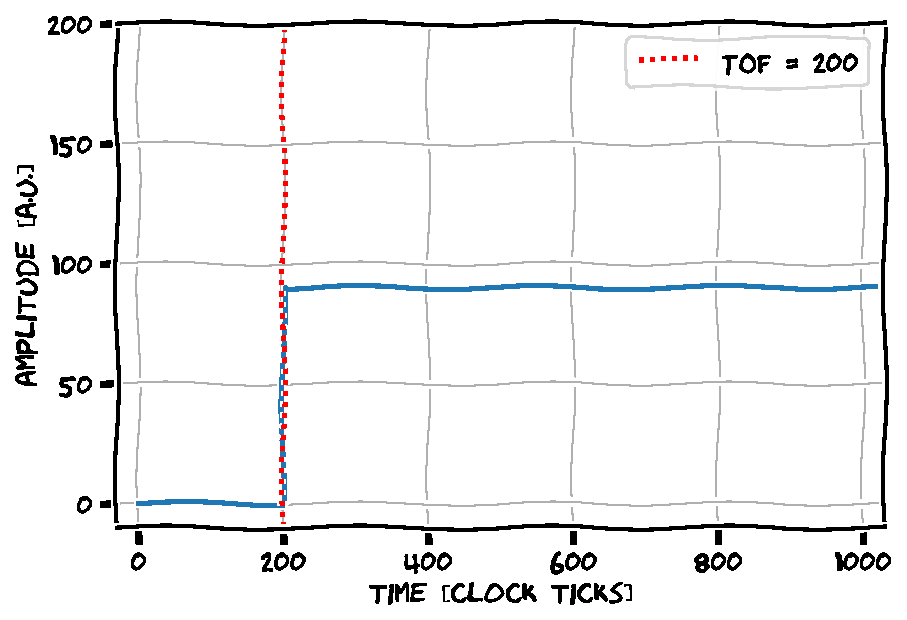
\includegraphics[width=8cm]{characterization/figures/time_of_flight_sketch.pdf}
    \caption{Plot of a generic time of flight experiment.}
    \label{fig:time_of_flight_sketch}
\end{figure}

Note that the unit of measurement for the x axis, the time axis, is in ADC \textit{clock ticks}.
This is because, in general, it is not really relevant the s/ns conversion~\footnote{In any case, we roughly have $4\text{ clock ticks} \approx 1$ ns}.

Of course, the plot presented in \cref{fig:time_of_flight_sketch} is an ideal one: in a real case scenario, we will have a much noisier signal and the edges of the rectangular pulse (both the rising and falling edges) will never appear "vertical").\\
To counter the effect of noise, we can repeat the experiment multiple times (usually called \textit{shots}), averaging the acquired waveforms.
We can also increase the initial amplitude of the pulse, however this has to be done carefully, since too much power could damage the components.\\
In any case, it is not important to be extremely precise with the time of flight estimation.

Note, anyway, that this experiment can be done with much more precision in later stages of the characterization: in particular after finding the resonator frequency.\\
Consider for example a system with a cavity, if we send through it a pulse that is not on resonance, the signal will mostly get absorbed and the acquired wave will need a lot of averages to become clearer.
If we know the exact resonator frequency, on the other hand, the signal will be highly amplified and the experiment will be easier.

In \cref{fig:time_of_flight} a real plot is presented.
We can see that the tone we sent (in this case at the resonator frequency) some effects can happen that distort the signal. 
However the shape sketched in \cref{fig:time_of_flight_sketch} is still clearly visible.\\
From this, a TOF value of 200 was chosen as the time offset between readout pulse firing and acquisition.

\begin{figure}[ht]
    \makebox[\textwidth][c]{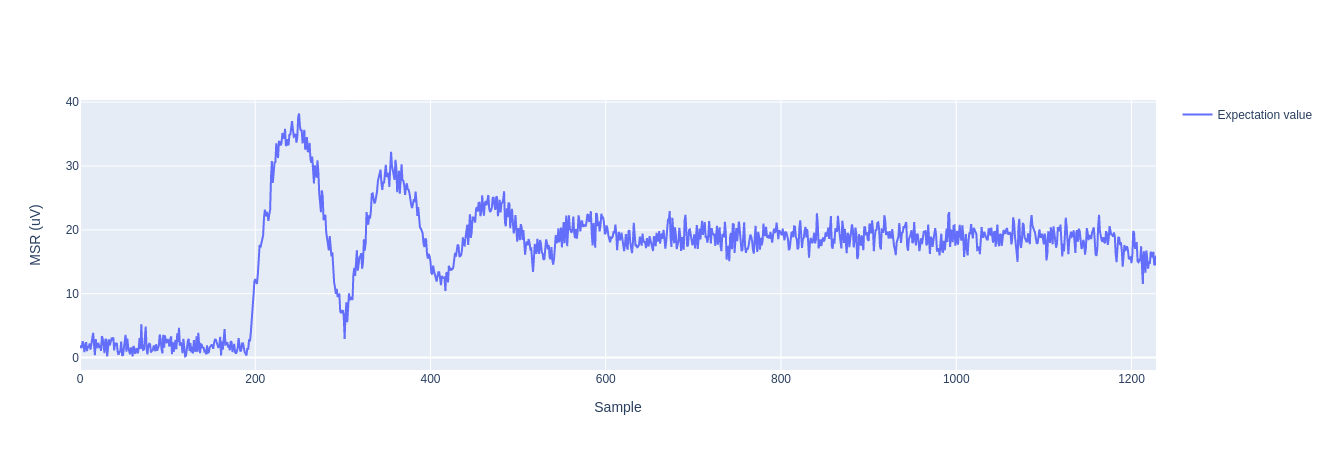
\includegraphics[width=1.3\textwidth]{characterization/figures/time_of_flight.png}}
    \caption{Plot of a time of flight experiment.}
    \label{fig:time_of_flight}
\end{figure}

The oscillating effect present in \cref{fig:time_of_flight} has different possible explanation, but can sometimes be linked to the use of a frequency (for the pulse) just slightly different from the resonance one.
In this case, the signal is amplified but with an initial detuning effect.
For a cavity, when this detuning is missing, we can expect something like \cref{fig:time_of_flight_2}, where we can see the characteristic charging and discharging effect of the cavity that behaves as a capacitor.

\begin{figure}[ht]
    \makebox[\textwidth][c]{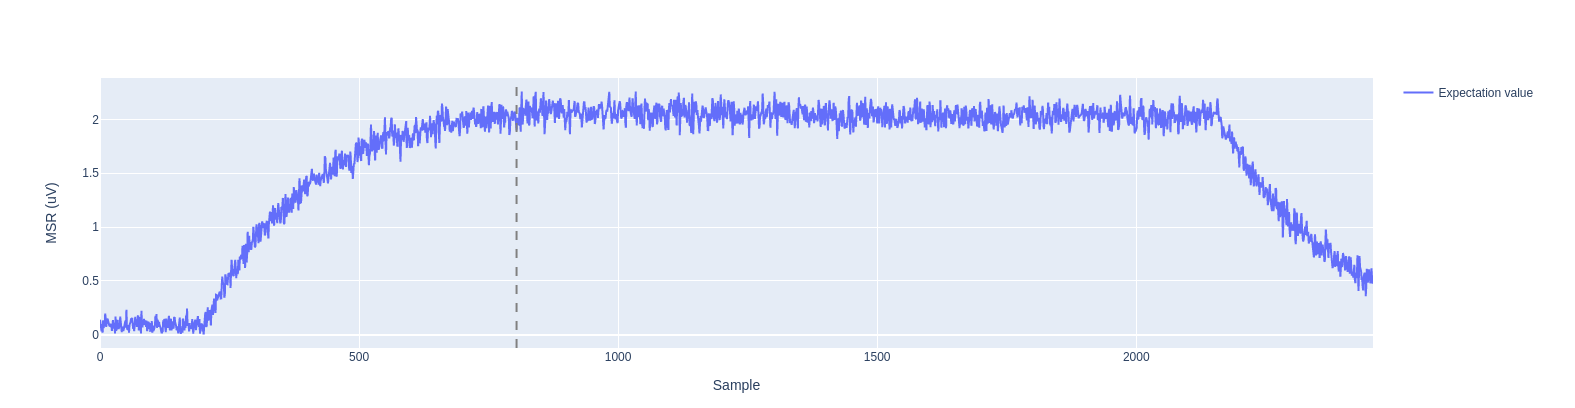
\includegraphics[width=1.3\textwidth]{characterization/figures/time_of_flight_2.png}}
    \caption{Plot of a time of flight experiment. the vertical line is merely the effect of a badly implemented fitting procedure.}
    \label{fig:time_of_flight_2}
\end{figure}

\experimentrecap
{Measurement Time of Flight}
{readout calibration}
{time of flight (adc offset)}
{a readout pulse gets fired, the ADC acquisition starts immediately. We plot acquired amplitude Vs time, we extract the TOF as the time where we visibly see a change in amplitude}